% Activate the following line by filling in the right side. If for example the name of the root file is Main.tex, write
% "...root = Main.tex" if the chapter file is in the same directory, and "...root = ../Main.tex" if the chapter is in a subdirectory.
 
%!TEX root =  ../Thesis.tex

\chapter[Fit Strategy and Results]{Fit Strategy and Results}

\subsection{Fit Model and Categories}
\label{subsec:fitmodel}

The statistical analysis of the data employs an unbinned likelihood
function, defined as:
\begin{equation}
\text{Pois}(N|\mu S+B) \prod_{k=1}^{njet\ cat} \prod_{l=1}^{N_{tag\ cat}} \prod_{i=1}^{N_{l}} \left[ \mu N_{S,k,l} PDF_{sig,k,l}(m_{bb,i}) + N_{B,k,l} PDF_{bkg}(m_{bb,i}) \right]
\end{equation}
where:
\begin{itemize}
\item the product is over the $b$-tag categories $l$, the n$_{jets}$ categores $k$, and over the events in each category $i$;
\item $N_{S,l}$ and $N_{B,l}$ are the expected signal and background yield in each category;
\item $PDF_{sig,l}(m_{bb})$ and $PDF_{bkg}(m_{bb})$ are the signal and background probability density functions for  the different categories;
\item $\mu$ is a signal strength which multiplies the overall signal prediction.
\end{itemize}


The $b$-tag fit categories $l$ are three exclusive categories to which events are assigned
based on the $b$-tag value of the third-most $b$-jet-like jet in the event (the two most
$b$-like jets have already been $b$-tagged in the trigger, and are assumed to be true
$b$-jets).  Then the categorization in $b$-tag fit categories splits the sample into three
regions with different signal and background enrichments:


\begin{itemize}
    \item bbb: one or more jets (in addition to the two triple-tagged jets) passing a tight (60\% working point)
 MV1 cut–-in effect, the full signal selection criteria
    \item bbloose: events failing the bbb classification but which have one or more jets passing a loose (80\%
working point) MV1 cut
    \item bbanti: events that have no jets passing an 80\% MV1 cut-–effectively a veto on the presence of any
b-tagged jets other than those firing the trigger
\end{itemize}

When assigning events to one of these categories, we only allow $b$-tags on the leading
five jets to count toward the bbb or bbloose categories.  In other words, if the third
$b$-tagged jet in an event is the 6th jet (in $p_T$ ordering) overall, the event 
will be classified as bbanti.  This requirement is motivated by our physics awareness that
the $b$-jets coming from signal events should be fairly high $p_T$, so this should have
a minimal effect of rejecting signal that would otherwise be accepted.  On the other
hand, with high-jet-multiplicity QCD events, there is the combinatorial effect of looking across
more jets for $b$-tags that increases the likelihood of an event being classified as signal-like
(bbb or bbloose) as there are more jets in the event.  Only looking at the leading 5 jets
for $b$-tags keeps this effect under control. 


The second type of categorization is based on the number of 
jets in the event: 3, 4, or 5 or more jets.  We find that the signal
shape can change based on the number of events, as well as the overall
signal and background normalizations. 




\subsection{PDF Shapes and Fit Constraints}
\label{sec:pdfs}

The background is fit with Bernstein polynomial.  A Bernstein polynomial of degree $n$ is
defined by

\begin{equation}
B_{i,n}(t) = n\choose{i} t^i (1-t)^{n-i}
\end{equation}

for $i=0,1,...,n$, where

\begin{equation}
n\choose{i} = \frac{n!}{i!(n-i)!}
\end{equation}

and there are $n+1$ polynomials of degree $n$.  Bernstein polynomials have the nice property
that they are guaranteed to always have positive values, as well as a reputation for
converging more easily than some other families of polynomials.

The exact degree of the polynomial is a free parameter to be chosen.  We inspect $n$ values
of 3, 4, and 5.



%http://www.slac.stanford.edu/econf/C0303241/proc/pres/502.PDF

\begin{figure}[phtb!]
  \begin{center}
  \begin{subfigure}[$m_{A}=400$ GeV]{0.4\textwidth}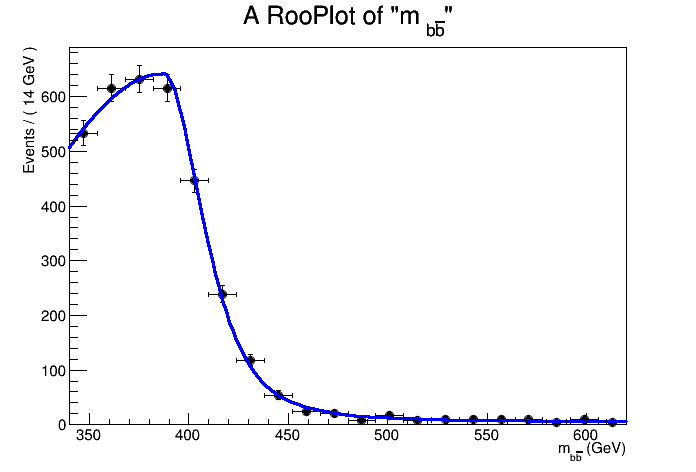
\includegraphics[width=\textwidth]{FitResults/images/fitMC_bAbb400_1.png}\end{subfigure}
  \begin{subfigure}[$m_{A}=450$ GeV]{0.4\textwidth}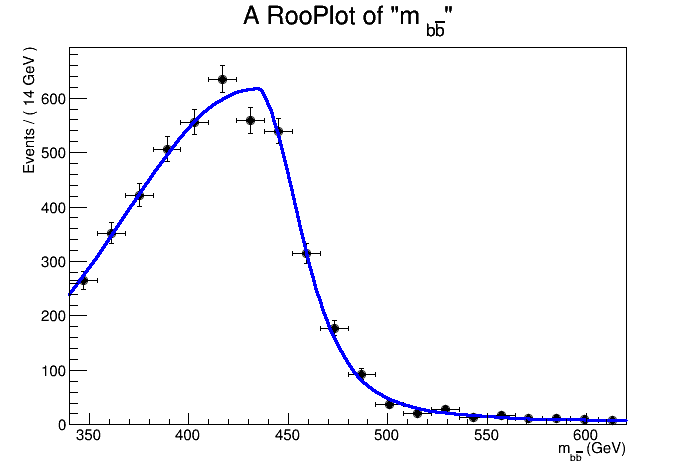
\includegraphics[width=\textwidth]{FitResults/images/fitMC_bAbb450_1.png}\end{subfigure}
  \begin{subfigure}[$m_{A}=500$ GeV]{0.4\textwidth}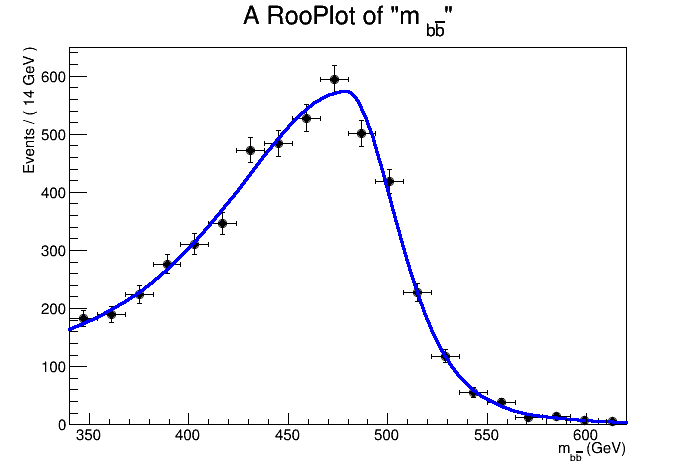
\includegraphics[width=\textwidth]{FitResults/images/fitMC_bAbb500_1.png}\end{subfigure}
  \begin{subfigure}[$m_{A}=550$ GeV]{0.4\textwidth}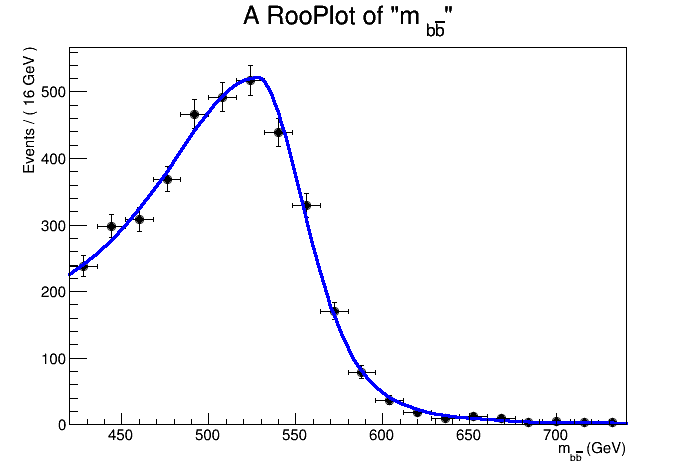
\includegraphics[width=\textwidth]{FitResults/images/fitMC_bAbb550_1.png}\end{subfigure}
  \begin{subfigure}[$m_{A}=600$ GeV]{0.4\textwidth}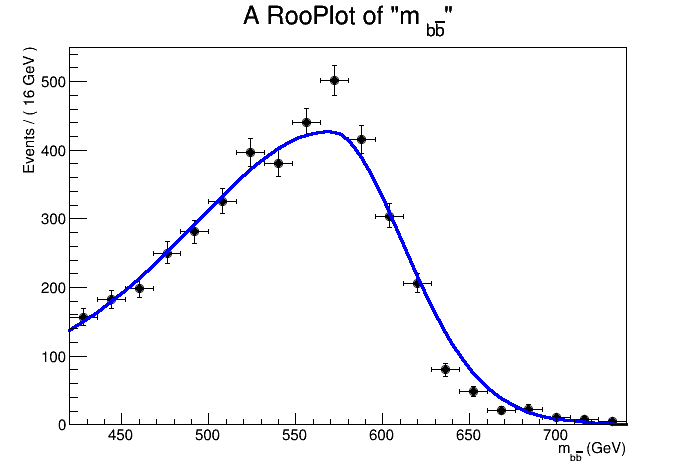
\includegraphics[width=\textwidth]{FitResults/images/fitMC_bAbb600_1.png}\end{subfigure}
  \begin{subfigure}[$m_{A}=650$ GeV]{0.4\textwidth}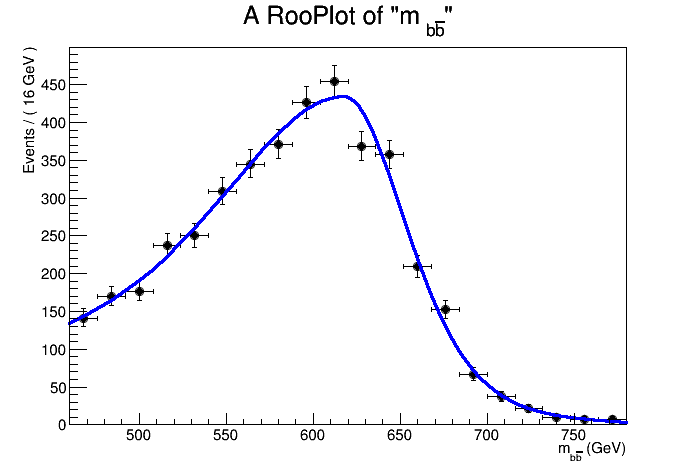
\includegraphics[width=\textwidth]{FitResults/images/fitMC_bAbb650_1.png}\end{subfigure}
  \begin{subfigure}[$m_{A}=700$ GeV]{0.4\textwidth}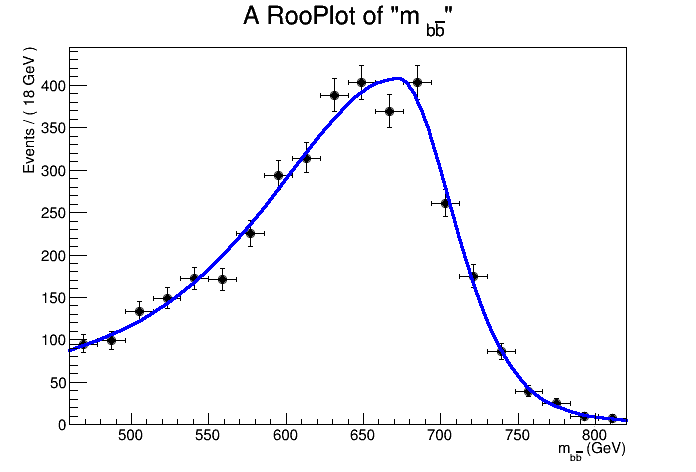
\includegraphics[width=\textwidth]{FitResults/images/fitMC_bAbb700_1.png}\end{subfigure}
  \begin{subfigure}[$m_{A}=800$ GeV]{0.4\textwidth}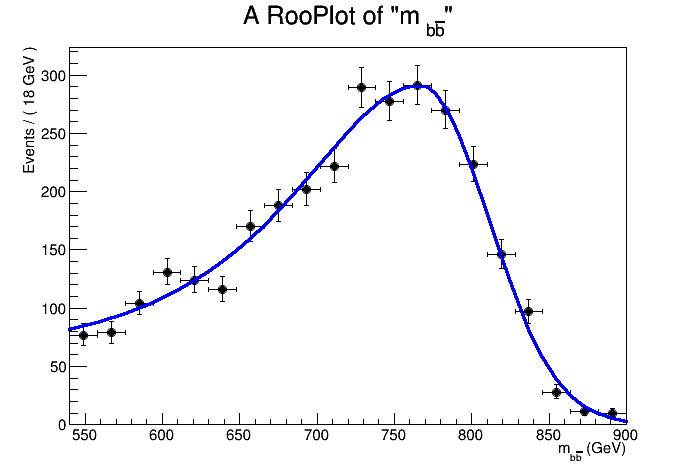
\includegraphics[width=\textwidth]{FitResults/images/fitMC_bAbb800_1.png}\end{subfigure}
  \caption{Signal PDFs for $m_{bb}$ in the {\it bbb} category, for events with 3 jets, for different $H/A$ masses. \label{fig:signalPDFs_3j}}
    \end{center}
\end{figure}


\begin{figure}[phtb!]
  \begin{center}
  \begin{subfigure}[$m_{A}=400$ GeV]{0.4\textwidth}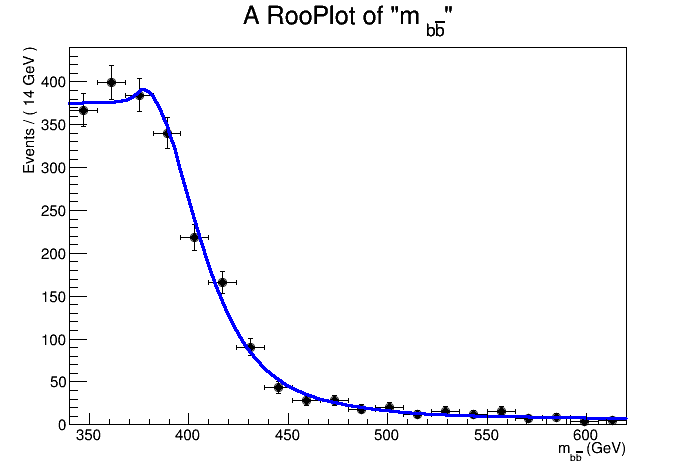
\includegraphics[width=\textwidth]{FitResults/images/fitMC_bAbb400_2.png}\end{subfigure}
  \begin{subfigure}[$m_{A}=450$ GeV]{0.4\textwidth}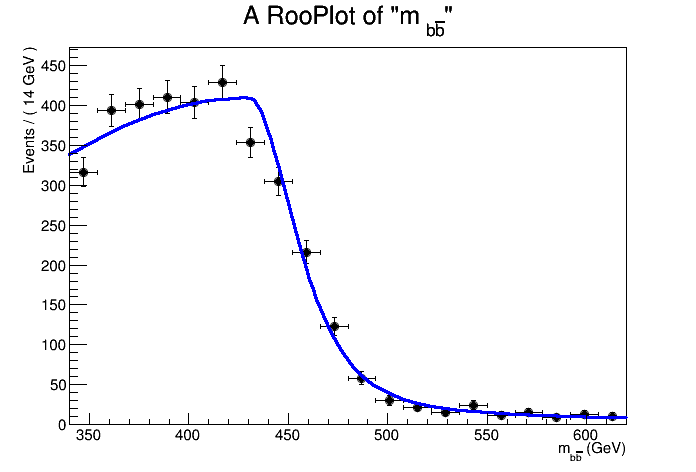
\includegraphics[width=\textwidth]{FitResults/images/fitMC_bAbb450_2.png}\end{subfigure}
  \begin{subfigure}[$m_{A}=500$ GeV]{0.4\textwidth}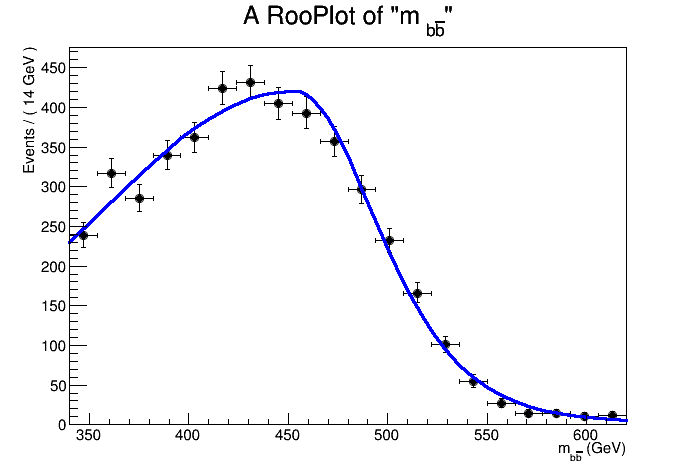
\includegraphics[width=\textwidth]{FitResults/images/fitMC_bAbb500_2.png}\end{subfigure}
  \begin{subfigure}[$m_{A}=550$ GeV]{0.4\textwidth}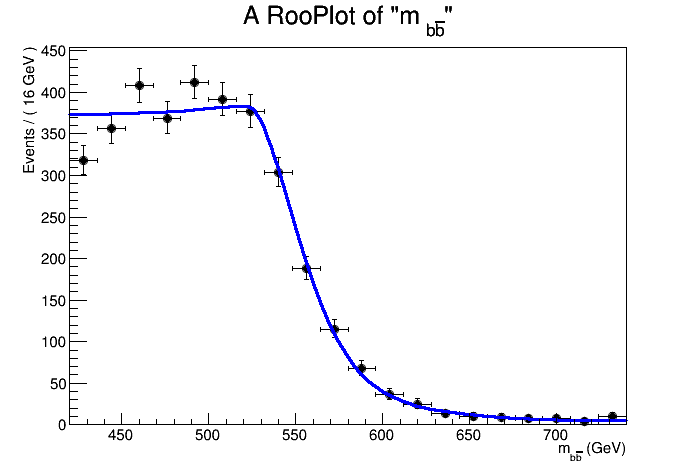
\includegraphics[width=\textwidth]{FitResults/images/fitMC_bAbb550_2.png}\end{subfigure}
  \begin{subfigure}[$m_{A}=600$ GeV]{0.4\textwidth}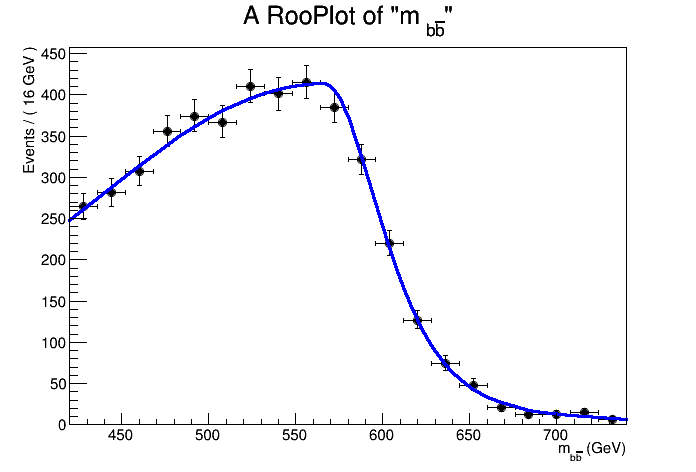
\includegraphics[width=\textwidth]{FitResults/images/fitMC_bAbb600_2.png}\end{subfigure}
  \begin{subfigure}[$m_{A}=650$ GeV]{0.4\textwidth}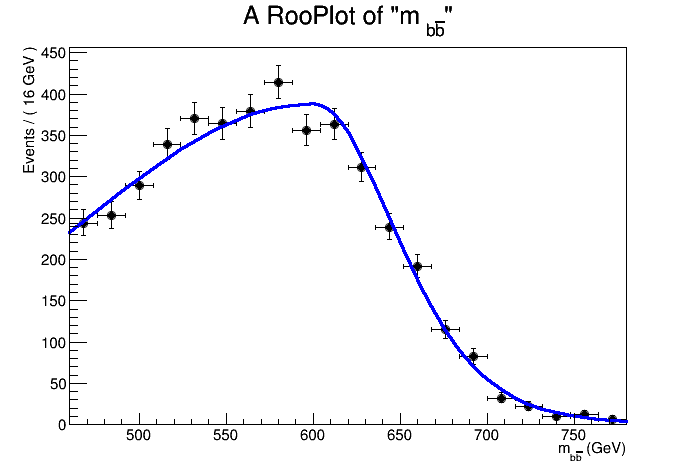
\includegraphics[width=\textwidth]{FitResults/images/fitMC_bAbb650_2.png}\end{subfigure}
  \begin{subfigure}[$m_{A}=700$ GeV]{0.4\textwidth}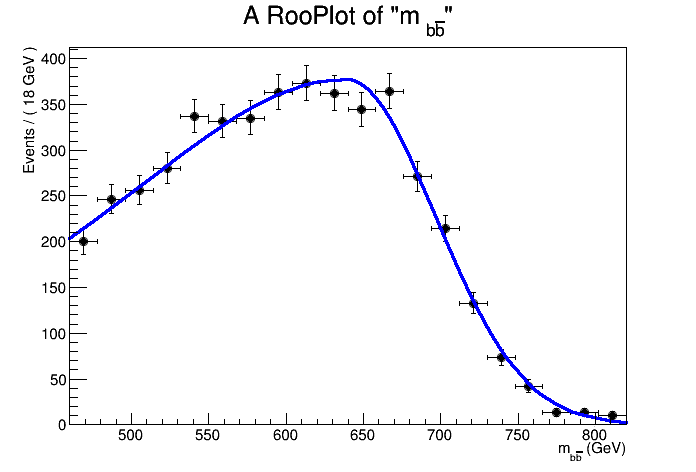
\includegraphics[width=\textwidth]{FitResults/images/fitMC_bAbb700_2.png}\end{subfigure}
  \begin{subfigure}[$m_{A}=800$ GeV]{0.4\textwidth}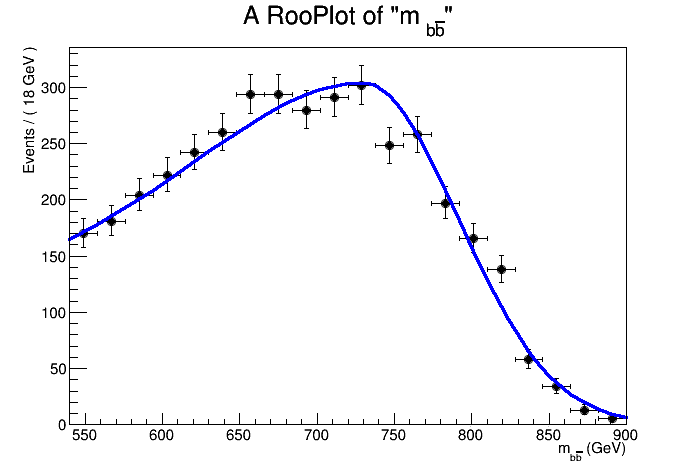
\includegraphics[width=\textwidth]{FitResults/images/fitMC_bAbb800_2.png}\end{subfigure}
  \caption{Signal PDFs for $m_{bb}$ in the {\it bbb} category, for events with 4 jets, for different $H/A$ masses. \label{fig:signalPDFs_4j}}
    \end{center}
\end{figure}


\begin{figure}[phtb!]
  \begin{center}
  \begin{subfigure}[$m_{A}=400$ GeV]{0.4\textwidth}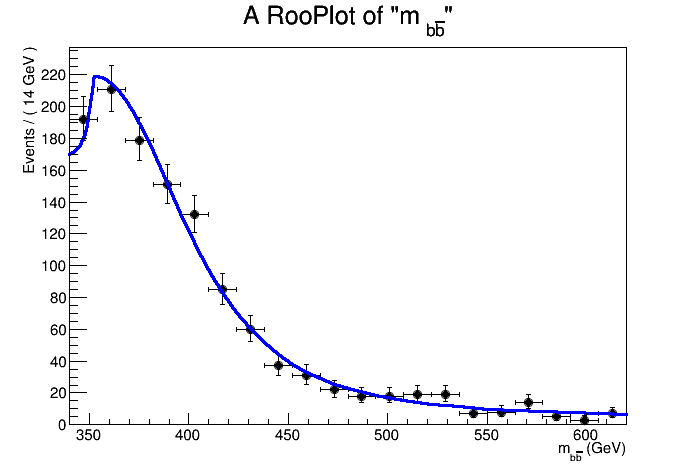
\includegraphics[width=\textwidth]{FitResults/images/fitMC_bAbb400_3.png}\end{subfigure}
  \begin{subfigure}[$m_{A}=450$ GeV]{0.4\textwidth}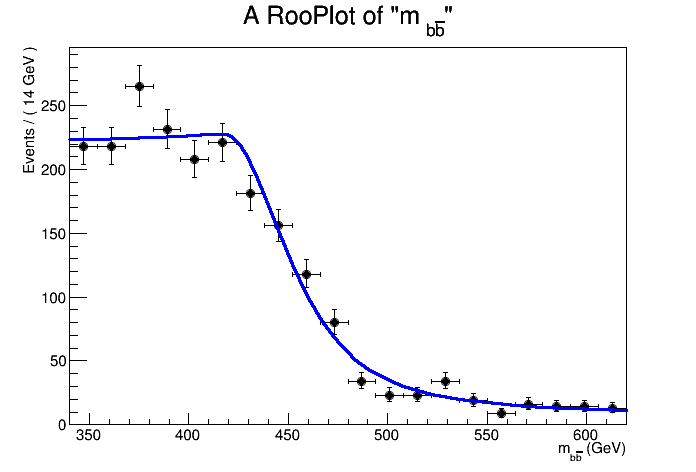
\includegraphics[width=\textwidth]{FitResults/images/fitMC_bAbb450_3.png}\end{subfigure}
  \begin{subfigure}[$m_{A}=500$ GeV]{0.4\textwidth}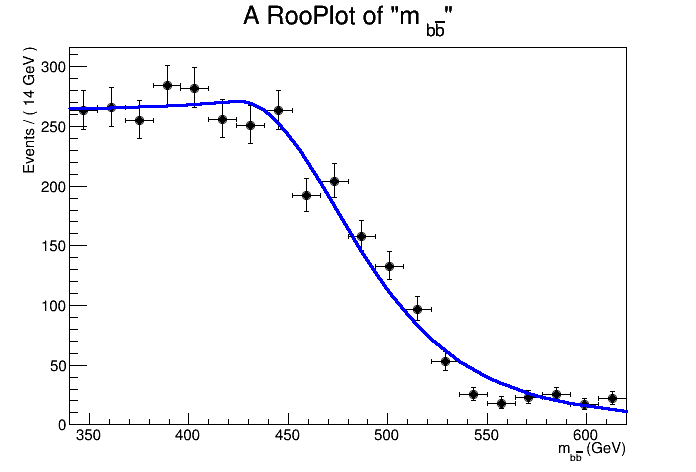
\includegraphics[width=\textwidth]{FitResults/images/fitMC_bAbb500_3.png}\end{subfigure}
  \begin{subfigure}[$m_{A}=550$ GeV]{0.4\textwidth}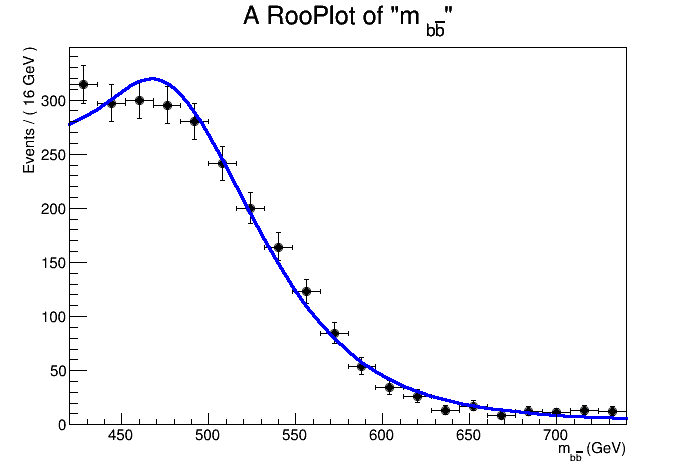
\includegraphics[width=\textwidth]{FitResults/images/fitMC_bAbb550_3.png}\end{subfigure}
  \begin{subfigure}[$m_{A}=600$ GeV]{0.4\textwidth}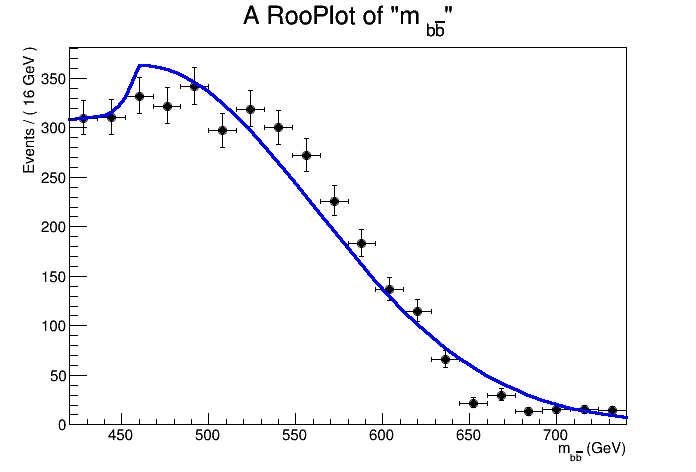
\includegraphics[width=\textwidth]{FitResults/images/fitMC_bAbb600_3.png}\end{subfigure}
  \begin{subfigure}[$m_{A}=650$ GeV]{0.4\textwidth}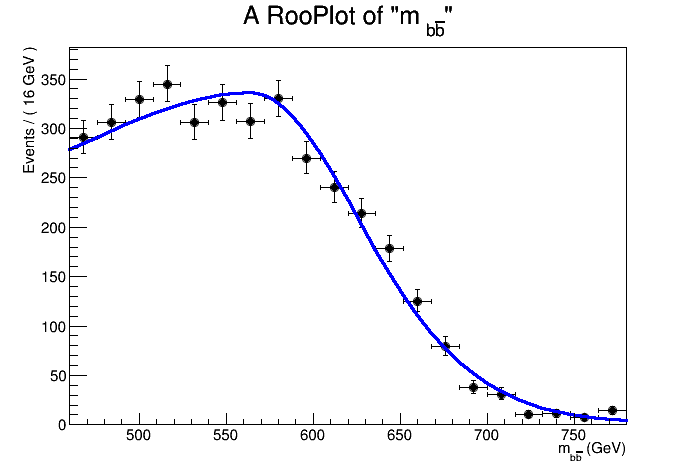
\includegraphics[width=\textwidth]{FitResults/images/fitMC_bAbb650_3.png}\end{subfigure}
  \begin{subfigure}[$m_{A}=700$ GeV]{0.4\textwidth}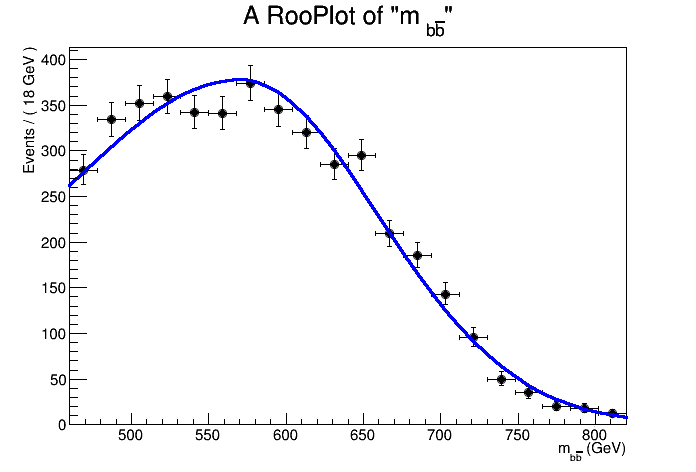
\includegraphics[width=\textwidth]{FitResults/images/fitMC_bAbb700_3.png}\end{subfigure}
  \begin{subfigure}[$m_{A}=800$ GeV]{0.4\textwidth}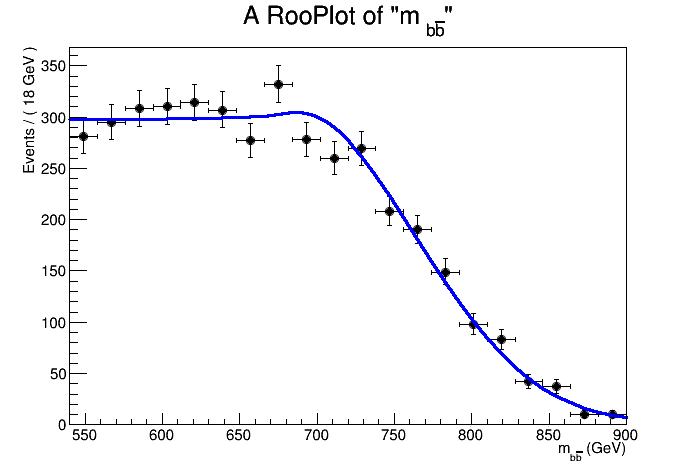
\includegraphics[width=\textwidth]{FitResults/images/fitMC_bAbb800_3.png}\end{subfigure}
  \caption{Signal PDFs for $m_{bb}$ in the {\it bbb} category, for events with 5 or more jets, for different $H/A$ masses. \label{fig:signalPDFs_5j}}
    \end{center}
\end{figure}



\section{Fit Yields}
\begin{table}
\caption{The $m_{bb}$ windows, predicted yields, and integrals for each of the
    mass points quantified with the fit. \label{tab:bkg_fit_yields}}
    \begin{tabular}{ c c c c c }
        $m_A$ & window low edge & window high edge & prediction & integral \\
    \end{tabular}
\end{table}


\section{Expected Sensitivity}


